\documentclass[12pt]{article} 
\usepackage[T1]{fontenc}
\usepackage[utf8]{inputenc} 
\usepackage[serbian]{babel} 
\usepackage{lmodern} 
\usepackage[expansion=false]{microtype} 
\usepackage{amsmath, amsthm, amssymb} 
\usepackage{graphicx} 
\usepackage{subfigure} % za \subfigure komandu 
\usepackage{tikz} 
\usepackage{dblfloatfix} 
\usepackage{tabto} 
\usepackage{float} 
\usepackage{booktabs} 
\usepackage{multirow} 
\usepackage{tikz}
\usetikzlibrary{trees}

\usepackage{tabularx} 
\usepackage{newtxtext}
\usepackage{diagbox}
\usepackage{capt-of} % u preambuli
\usepackage{hyperref}


\usepackage[a4paper, left=2cm, right=2cm, top=2.5cm, bottom=2.5cm]{geometry}
\renewcommand{\baselinestretch}{1.0} 
\usepackage{enumitem}  


\renewcommand{\refname}{Literatura}
\usepackage[nottoc]{tocbibind}

\setcounter{page}{1}
\title{Modelovanje i predikcija koncentracija polena u Srbiji korišćenjem geostatistike i mašinskog učenja}
\author{Luka Milutinović}
\date{Univerzitet u Beogradu, Elektrotehnički fakultet, 2025.}
\begin{document}
\newpage

\begin{figure}[H]
    \centering
    
\includegraphics[width=2cm]{grafici/etflogotip.png}

\end{figure}

\begin{center}
\large \textbf{UNIVERZITET U BEOGRADU}
\end{center}
\begin{center}
\large \textbf{ELEKTROTEHNIČKI FAKULTET}
\end{center}



\thispagestyle{empty}


\vspace*{3cm}
\begin{center}
\Huge \textbf{Predikcija dnevne prodaje u Rossmann prodavnicama primenom metoda mašinskog učenja}
\end{center}


\begin{center}
\small \textbf{Projekat iz mašinskog učenja}
\end{center}


\vspace*{6cm}

\begin{center}
\hspace*{9cm}\large\textsl{student} \newline
\hspace*{8cm}\large \textbf{Luka Milutinović 2021/0103}\newline
\end{center}


\vspace*{0.9cm}

\begin{center}
\normalsize	 BEOGRAD,  2026.
\end{center}

\mbox{}
\newpage
\thispagestyle{empty}
\tableofcontents
\thispagestyle{empty}
\mbox{}
\newpage
\setcounter{page}{1}
\section{Uvod i opis problema}

Rossmann je jedan od vodećih lanaca drogerija u Evropi, sa više od 3.000 prodavnica raspoređenih u sedam zemalja. Svaka prodavnica svakodnevno beleži prodaju i menadžeri su odgovorni da planiraju buduće potrebe, uključujući broj zaposlenih i zalihe, čak do šest nedelja unapred. Predviđanje prodaje nije jednostavno: na nju utiče mnogo faktora kao što su promocije, konkurencija, praznici i lokacija prodavnice. Zbog toga se tačnost predikcija može znatno razlikovati između prodavnica.

U okviru takmičenja na platformi \textit{Kaggle} (\href{https://www.kaggle.com/competitions/rossmann-store-sales}{\textit{Rossmann Store Sales}}), zadatak je da se predvidi šest nedelja dnevne prodaje za 1.115 prodavnica u Nemačkoj. Pouzdane prognoze pomažu menadžerima da bolje planiraju radnu snagu i optimizuju zalihe, čime se poboljšava efikasnost i zadovoljstvo kupaca.

U skupu podataka dostupni su sledeći atributi:

\begin{itemize}
    \item \textbf{Id} – jedinstveni identifikator koji predstavlja kombinaciju (\texttt{Store}, \texttt{Date}) u test skupu. Koristi se samo za praćenje predikcija, nema uticaja na model.
    
    \item \textbf{Store} – jedinstveni identifikator svake prodavnice.
    
    \item \textbf{Sales} – dnevni prihod prodavnice. 
    
    \item \textbf{Customers} – broj kupaca koji su posetili prodavnicu tog dana.
    \item \textbf{Open} – indikator da li je prodavnica bila otvorena (1 = otvorena, 0 = zatvorena).
    
    \item \textbf{StateHoliday} – tip državnog praznika na datom datumu. Oznake su: \texttt{a} = javni praznik, \texttt{b} = Uskrs, \texttt{c} = Božić, \texttt{0} = nema praznika. 
    
    \item \textbf{SchoolHoliday} – indikator zatvorenosti škola u datom periodu (1 = da, 0 = ne). 
    
    \item \textbf{StoreType} – klasifikacija prodavnica u četiri tipa: a, b, c, d. Svaki tip ima različitu veličinu, asortiman i ciljnu publiku.
    
    \item \textbf{Assortment} – nivo asortimana: \texttt{a} = osnovni, \texttt{b} = prošireni, \texttt{c} = kompletni.
    
    \item \textbf{CompetitionDistance} – udaljenost najbližeg konkurentskog objekta u metrima. 
    \item \textbf{CompetitionOpenSinceMonth / CompetitionOpenSinceYear} – mesec i godina kada je najbliži konkurent otvoren. 
    
    \item \textbf{Promo} – indikator da li je prodavnica tog dana imala aktivnu promotivnu kampanju (1 = da, 0 = ne). 
    
    \item \textbf{Promo2} – indikator kontinualnih i ponovljenih promocija za određene prodavnice (1 = prodavnica učestvuje, 0 = ne učestvuje). 
    
    \item \textbf{Promo2SinceYear / Promo2SinceWeek} – godina i nedelja kada je prodavnica počela sa Promo2 kampanjom. 
    
    \item \textbf{PromoInterval} – meseci u kojima se promocija ponavlja.
    
    \item \textbf{Date} – datum za koji je zabeležena prodaja.
\end{itemize}


Evalucija predikcija vrši se korišćenjem metrike \textbf{Root Mean Square Percentage Error (RMSPE)}, koja meri relativnu grešku predikcija u odnosu na stvarnu prodaju:

\[
RMSPE = \sqrt{\frac{1}{n} \sum_{i=1}^{n} \left( \frac{y_i - \hat{y}_i}{y_i} \right)^2}
\]

Pri tome se dani i prodavnice sa nulom prodaje izuzimaju iz izračunavanja greške.  

Cilj ovog projekta je razviti modele koji mogu precizno predvideti dnevnu prodaju, koristeći istorijske podatke i informacije o prodavnicama, kako bi menadžeri mogli da donose bolje odluke i efikasnije planiraju resurse.


\newpage

\section{Eksplorativna analiza podataka (EDA)}

Eksplorativna analiza podataka sprovedena je kako bi se utvrdila struktura skupa, uočile sezonalnosti, korelacije i eventualni problemi u podacima.

\subsection{Osnovne karakteristike podataka}

Podaci su organizovani u tri odvojena skupa:

\begin{itemize}
    \item \textbf{Trening skup} (\texttt{train}): sadrži istorijske podatke o prodaji sa poznatim vrednostima ciljne promenljive \texttt{Sales}. Dimenzije skupa su $(1\,017\,209 \times 9)$.
    \item \textbf{Podaci o prodavnicama} (\texttt{store}): sadrže karakteristike prodavnica, uključujući tip prodavnice, asortiman, konkurenciju i promotivne informacije. Dimenzije ovog skupa su $(1\,115 \times 10)$.
    \item \textbf{Test skup} (\texttt{test}): sadrži podatke za koje je potrebno predvideti prodaju. Dimenzije su $(41\,088 \times 8)$, a period obuhvata 60 dana počevši od avgusta 2015. Vrednosti \texttt{Sales} nisu poznate.
\end{itemize}

Ciljna promenljiva u ovom problemu je \texttt{Sales}, dok ostale kolone predstavljaju različite karakteristike prodavnica i datume prodaje koje se koriste za modelovanje.


\subsection{Nedostajući podaci}

U skupu podataka uočeni su određeni nedostaci:  

\begin{itemize}
    \item Za tri prodavnice nedostajala je informacija o udaljenosti od najbližeg konkurenta. Ove vrednosti su popunjene medijanom udaljenosti ostalih prodavnica.
    \item Kod 354 prodavnice nije bio poznat datum kada je konkurentska prodavnica otvorena. Za ove slučajeve pretpostavlja se da konkurencija još nije otvorila svoje objekte.
    \item Za atribut \texttt{Promo2} nedostaju podaci o početku trajanja promocije kod prodavnica koje ne učestvuju u Promo2. Pošto se te informacije ne primenjuju na prodavnice koje nisu uključene, nije bilo potrebe za popunjavanjem.
    \item Postoji 3,15\% dana za koje prodaja nije zabeležena u skupu podataka. Za ove datume pretpostavljeno je da je prodaja iznosila 0, što je u skladu sa indikatorom \texttt{Open} i logikom poslovanja.
\end{itemize}
\newpage
\subsection{Analiza nulte prodaje}

U ovom skupu podataka, dani sa nultom prodajom nisu predmet analize i neće se koristiti pri treniranju modela. Većina slučajeva nulte prodaje (oko 17\%) odgovara danima kada prodavnica nije bila otvorena (\texttt{Open = 0}). Pored toga, u skupu podataka zabeleženo je još 54 dana sa nultom prodajom, što čini približno 0,005\% svih zapisa. S obzirom na izuzetno mali udeo ovih anomalija, odlučeno je da se oni ne analiziraju niti uključuju u treniranje modela.


\subsection{Statistika ciljne promenljive}

Ciljna promenljiva \texttt{Sales} pokazuje jaku asimetriju u raspodeli. Većina dana ima relativno malu prodaju, dok se u skupu podataka povremeno javljaju retki dani sa veoma visokim iznosima prodaje, što stvara tzv. „dugi rep“. Ova raspodela može otežati treniranje modela, jer ekstremne vrednosti značajno utiču na metrike greške i učenje.

\begin{figure}[h]
    \centering
    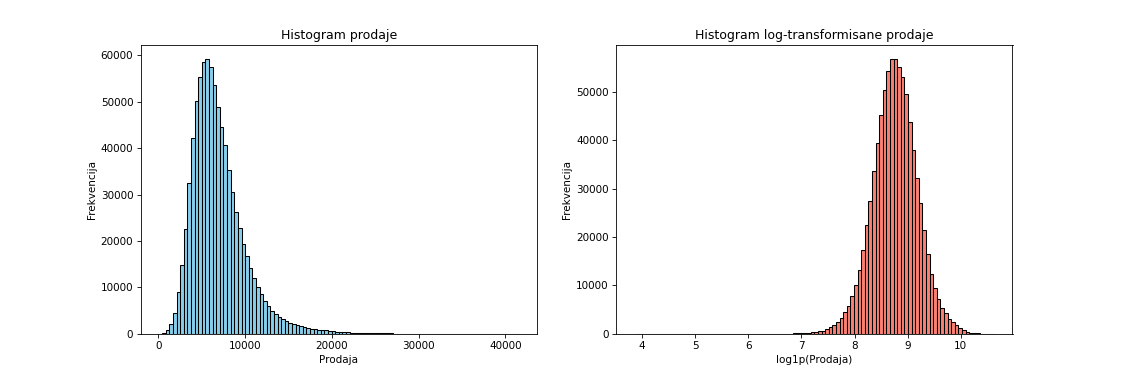
\includegraphics[width=1\textwidth]{grafici/sales_histogram.png}
    \caption{Levo: histogram originalne raspodele \texttt{Sales}. Desno: histogram \texttt{log1p(Sales)}, koji prikazuje ravnomerniju raspodelu vrednosti nakon log-transformacije.}
\end{figure}

Kako bi se smanjio uticaj ekstremnih vrednosti i „izravnala“ raspodela, primenjena je logaritamska transformacija, definisana kao:

\[
y' = \log(1 + y)
\]

Nakon primene logaritamske transformacije, distribucija vrednosti \texttt{Sales} postaje mnogo ujednačenija i gotovo da je poprimila oblik Gausove raspodele.


\subsection{Uticaj vremenskih i spoljašnjih faktora na prodaju}

U okviru istraživanja analizirani su različiti vremenski i spoljašnji faktori koji utiču na promene u prodaji.  
Posebna pažnja posvećena je uticaju promocija, sezonalnosti, tipa prodavnice, udaljenosti konkurencije i praznika, jer su to najčešći uzroci fluktuacija u prihodima maloprodajnih objekata.

\subsection*{Promocije i sezonalnost}

Rezultati jasno pokazuju da promocije imaju pozitivan uticaj na prodaju — tokom promotivnih perioda prosečna prodaja je u proseku viša za oko 30\% u odnosu na dane bez promocija.  

Što se tiče vremenskih obrazaca, analizirani su sledeći aspekti:

\textbf{Prodaja po godinama.}  
Na slici~\ref{fig:promo_by_year} prikazana je prosečna prodaja sa i bez promocija po godinama. Može se primetiti da ne postoji statistički značajna razlika u prosečnoj prodaji između različitih godina, što ukazuje na relativnu stabilnost tržišta u posmatranom periodu.

\begin{figure}[H]
    \centering
    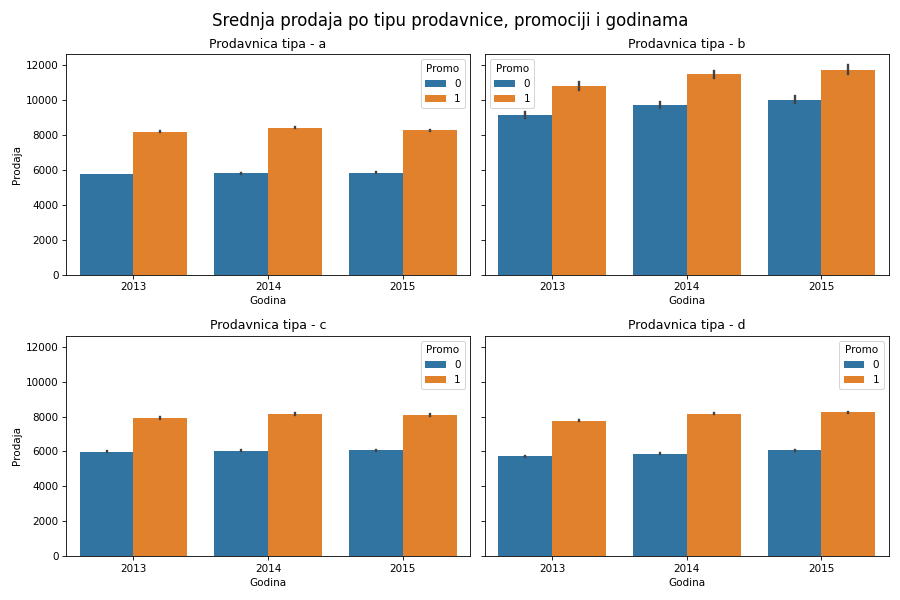
\includegraphics[width=0.8\textwidth]{grafici/promo_by_year.png}
    \caption{Prosečna prodaja sa i bez promocija po godinama.}
    \label{fig:promo_by_year}
\end{figure}

\textbf{Prodaja po mesecima.}  
Na slici~\ref{fig:promo_by_month} vidi se izražena sezonalnost, sa najvišom prodajom u decembru, što je očekivano zbog povećane potrošnje tokom praznične sezone.

\begin{figure}[H]
    \centering
    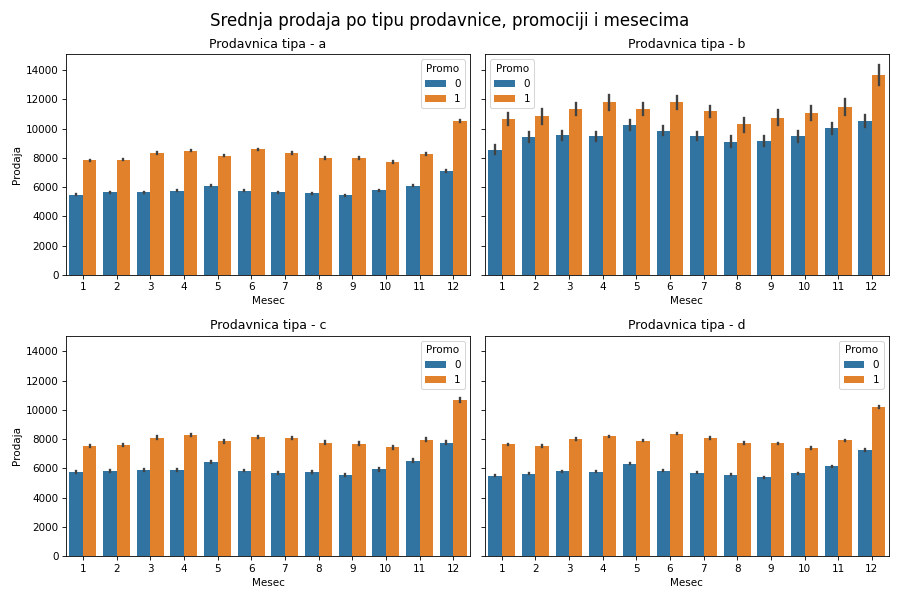
\includegraphics[width=0.8\textwidth]{grafici/promo_by_month.png}
    \caption{Prosečna prodaja sa i bez promocija po mesecima.}
    \label{fig:promo_by_month}
\end{figure}

\textbf{Prodaja po danima u nedelji.}  
Na slici~\ref{fig:promo_by_weekday} prikazana je prosečna prodaja po danima u nedelji. Prodaja je uglavnom najviša ponedeljkom, iako ovaj obrazac delimično zavisi od tipa prodavnice. Neki tipovi beleže povećanu prodaju i vikendom.

\begin{figure}[H]
    \centering
    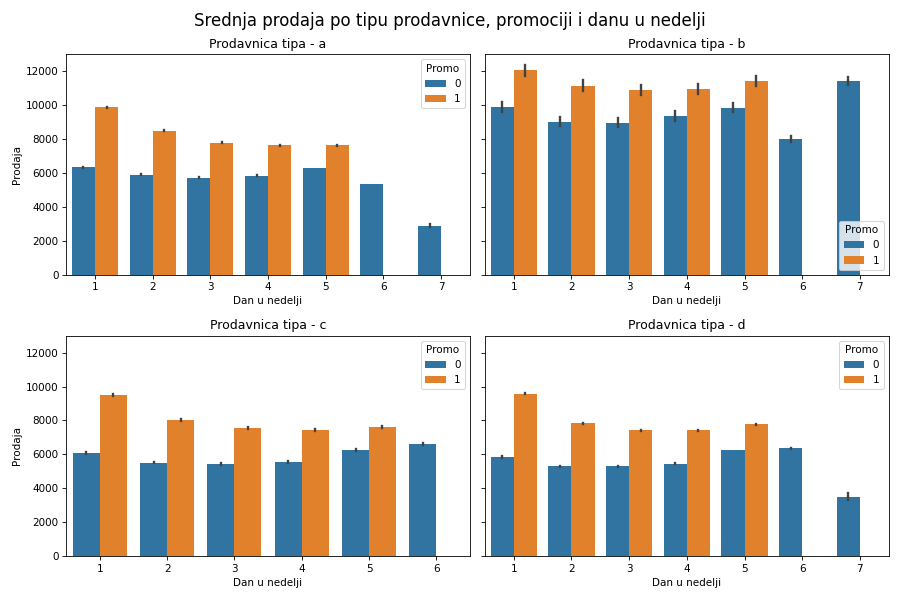
\includegraphics[width=0.8\textwidth]{grafici/promo_by_day.png}
    \caption{Prosečna prodaja sa i bez promocija po danima u nedelji.}
    \label{fig:promo_by_weekday}
\end{figure}

Kada je u pitanju struktura prodavnica, prodavnice tipa \texttt{b} beleže najveću prosečnu prodaju, dok su rezultati za ostale tipove (\texttt{a}, \texttt{c}, \texttt{d}) međusobno slični.

\subsubsection*{Dugoročne promocije (Promo2)}

Program \texttt{Promo2} predstavlja kontinuirane, ponavljajuće promocije koje se sprovode u određenim mesecima tokom godine.  
Analiza pokazuje da su ove promocije najčešće aktivne kod prodavnica sa nižom prosečnom prodajom, što verovatno odražava strategiju kompanije da podstakne promet kod slabije uspešnih objekata.  
Posebno je primetno da prodavnice tipa \texttt{a} i \texttt{d} imaju značajno smanjenu prosečnu prodaju.
Na slici~\ref{fig:promo2_avg} prikazana je prosečna prodaja u zavisnosti od prisustva programa \texttt{Promo2}.  


\begin{figure}[H]
    \centering
    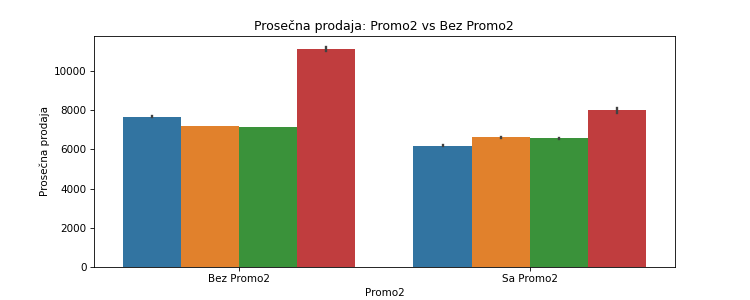
\includegraphics[width=0.8\textwidth]{grafici/promo2_avg_sales.png}
    \caption{Prosečna prodaja u zavisnosti od prisustva dugoročne promocije (\texttt{Promo2}).}
    \label{fig:promo2_avg}
\end{figure}

Na pojedinačnim primerima se vidi da efekat \texttt{Promo2} nije uvek izražen. Kod prodavnice sa ID-jem~11, na primer, prodaja je ostala gotovo nepromenjena i nakon uvođenja programa.
\begin{figure}[H]
    \centering
    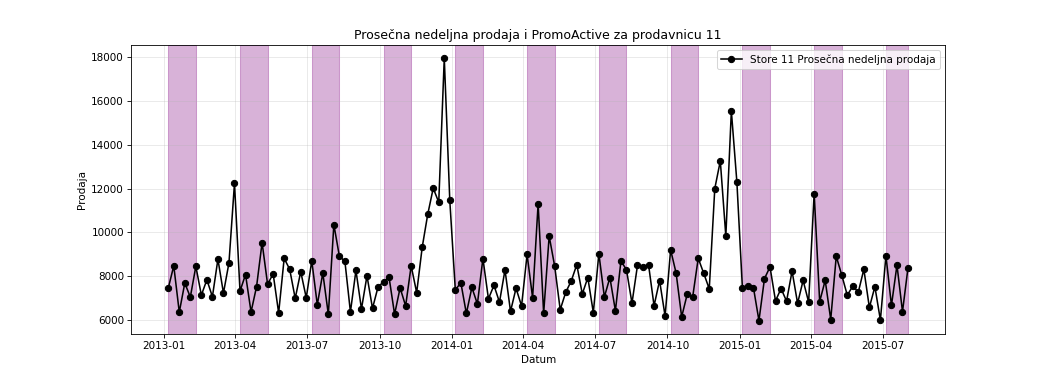
\includegraphics[width=0.96\textwidth]{grafici/promo2_example.png}
    \caption{Primer dinamike prodaje kod prodavnice sa aktivnim programom \texttt{Promo2} (prodavnica 11).}
    \label{fig:promo2_example}
\end{figure}

\subsubsection*{Udaljenost konkurencije}

Udaljenost konkurencije pokazuje jasan obrazac uticaja na prodaju.  
Kada je konkurencija veoma blizu, prodaja vidno opada, što sugeriše da kupci lako prelaze kod konkurenta.  
Kako se rastojanje povećava, ovaj efekat postaje sve slabiji, a kod većih distanci gotovo da nema primetnog uticaja na poslovanje.

Na slici~\ref{fig:competition_near} prikazan je primer prodavnice koja se nalazi u neposrednoj blizini konkurencije, gde se jasno vidi niža prosečna prodaja.  
Suprotno tome, na slici~\ref{fig:competition_far} prikazana je prodavnica koja je znatno udaljena od najbližeg konkurenta, kod koje se prodaja održava na stabilnom nivou.

\begin{figure}[H]
    \centering
    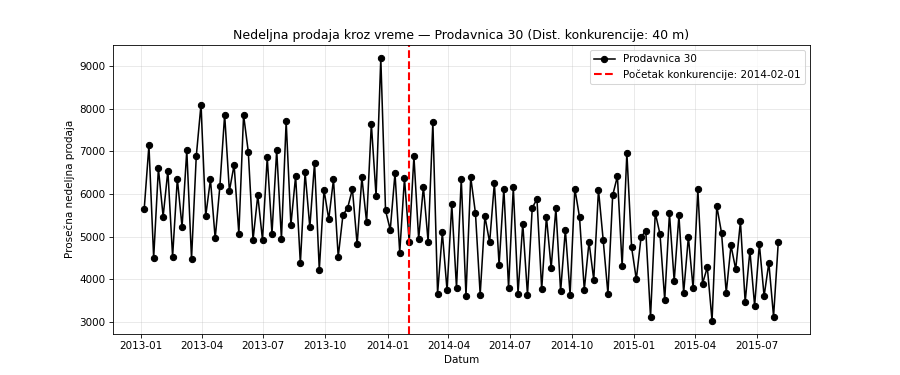
\includegraphics[width=0.96\textwidth]{grafici/competition_near.png}
    \caption{Prodavnica sa malom udaljenošću od konkurencije – uočljiv pad prodaje.}
    \label{fig:competition_near}
\end{figure}

\begin{figure}[H]
    \centering
    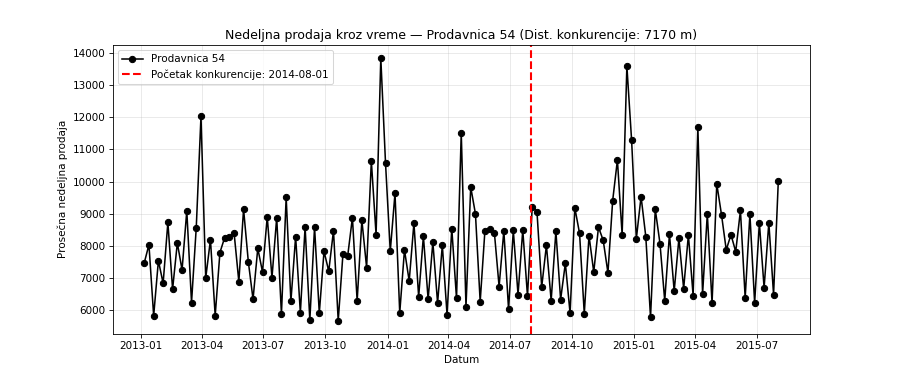
\includegraphics[width=0.96\textwidth]{grafici/competition_far.png}
    \caption{Prodavnica sa velikom udaljenošću od konkurencije – stabilna prodaja bez većih oscilacija.}
    \label{fig:competition_far}
\end{figure}

\subsection*{Praznici i školski raspusti}

Tokom praznika prodavnice različitih tipova pokazuju različite obrasce ponašanja.  
Prodavnice tipa \texttt{b} beleže primetan skok prodaje, dok kod tipova \texttt{a} i \texttt{d} dolazi do blagog pada.  
Prodavnice tipa \texttt{c} najčešće ne rade tokom praznika, pa je prodaja tada nula.  
Na slici~\ref{fig:holiday_effects} prikazan je uticaj praznika na prosečnu prodaju po tipu prodavnice.

\begin{figure}[H]
    \centering
    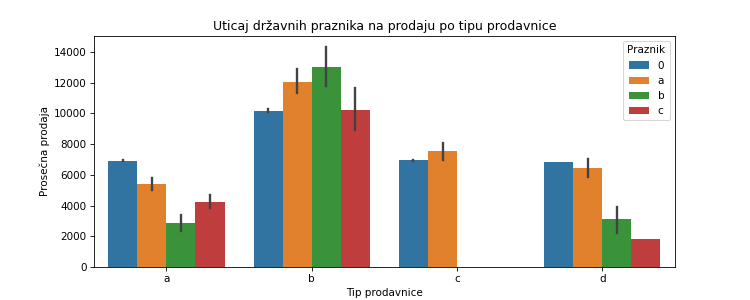
\includegraphics[width=0.9\textwidth]{grafici/holiday_effects.png}
    \caption{Uticaj praznika na prosečnu prodaju po tipu prodavnice.}
    \label{fig:holiday_effects}
\end{figure}

Tokom školskih raspusta uočava se blag porast prodaje kod većine prodavnica.  
Na slici~\ref{fig:school_holidays} prikazan je uticaj školskih raspusta na prosečnu prodaju.

\begin{figure}[H]
    \centering
    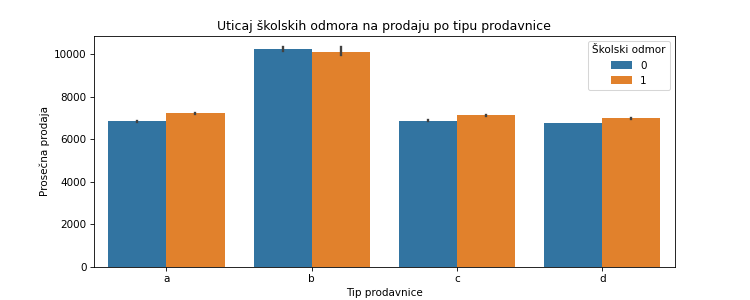
\includegraphics[width=0.9\textwidth]{grafici/school_holidays.png}
    \caption{Uticaj školskih raspusta na prosečnu prodaju po tipu prodavnice.}
    \label{fig:school_holidays}
\end{figure}


\subsection{Stacionarnost vremenskog signala}

Na osnovu prethodne analize karakteristika podataka jasno je da signal prodaje nije stacionaran — prosečna vrednost i varijansa menjaju se tokom vremena. Ovaj efekat je očekivan, jer podaci pokazuju izraženu sezonalnost, uticaj promocija, praznika i različitih tipova prodavnica.

Rezultati testova stacionarnosti dodatno potvrđuju ovu procenu.  
ADF test ne prepoznaje prisustvo jediničnog korena, dok KPSS test ukazuje na prisustvo slučajnog hoda.

Zbog nepostojanja stacionarnosti, linearni modeli zasnovani na pretpostavci stacionarnog signala, kao što su \texttt{SARIMAX} ili \texttt{Prophet}, nisu direktno primenljivi.  
Iako bi se serija mogla diferencirati kako bi postala stacionarna, takav postupak bi promenio osnovnu strukturu podataka i otežao modeliranje dana sa nultom prodajom.

Na slici~\ref{fig:acf_pacf_4x1} prikazana je kompletna analiza po tipu prodavnice (\texttt{a}–\texttt{d}). Svaki red predstavlja jedan tip prodavnice i sadrži tri kolone: vremenski signal, autokorelacionu funkciju (ACF) i parcijalnu autokorelacionu funkciju (PACF).  

Analiza vremenskih signala i ACF/PACF funkcija pokazuje sledeće obrasce:
\begin{itemize}
    \item Svi tipovi prodavnica pokazuju izraženu sezonalnost sa periodom od približno 7 dana, što odgovara nedeljnom obrascu kupovine.  
    Autokorelaciona funkcija (ACF) za prodavnice \texttt{a}, \texttt{c} i \texttt{d} pokazuje izražene pikove na 12. komponenti, dok prodavnice tipa \texttt{b} imaju dominantan pik na 7. komponenti.
    
    \item Parcijalna autokorelaciona funkcija (PACF) signalizira složenu strukturu vremenskog niza.  
    Za prodavnice tipa \texttt{a} i \texttt{b} primetan je pik na vremenskom kašnjenju od 7 dana, dok prodavnice \texttt{c} i \texttt{d} pokazuju izražen prvi pik.  
    Ovi obrasci ukazuju na različite kratkoročne i dugoročne zavisnosti po tipovima prodavnica.
\end{itemize}

Ovi uvidi ukazuju da je u daljoj analizi bolje koristiti modele koji ne zahtevaju strogu stacionarnost, kao što su regresioni i ansambl modeli, umesto klasičnih vremenskih serija.

\begin{figure}[H]
    \centering
    % Prva slika - tip a
    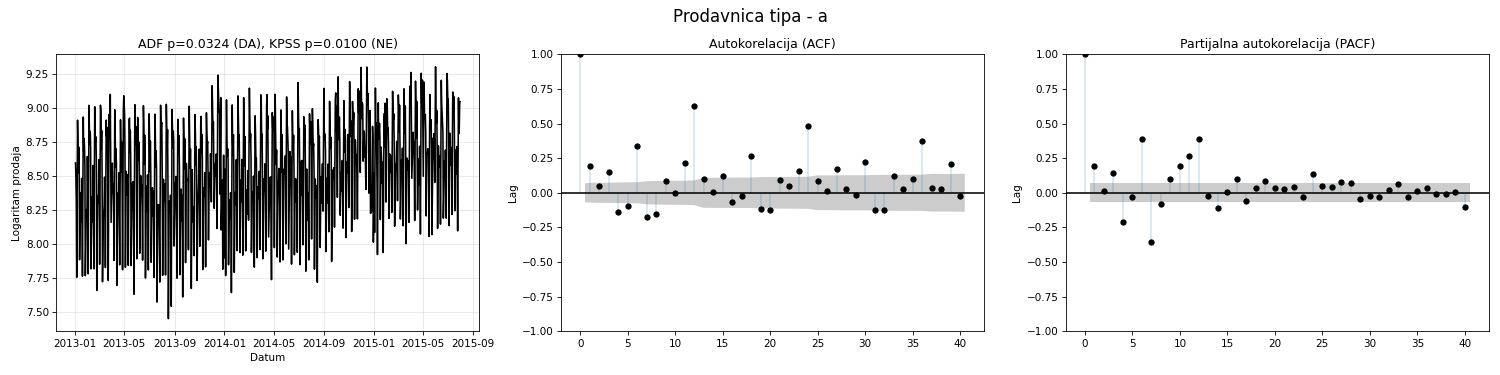
\includegraphics[width=0.9\textwidth]{grafici/store_a.png}
    \vspace{0.3cm}  % razmak između redova
    
    % Druga slika - tip b
    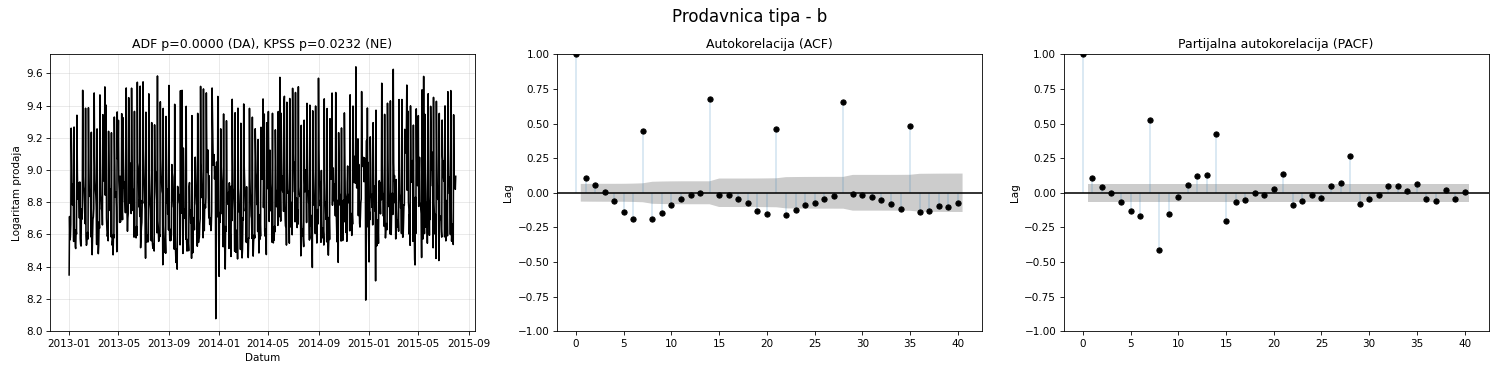
\includegraphics[width=0.9\textwidth]{grafici/store_b.png}
    \vspace{0.3cm}
    
    % Treća slika - tip c
    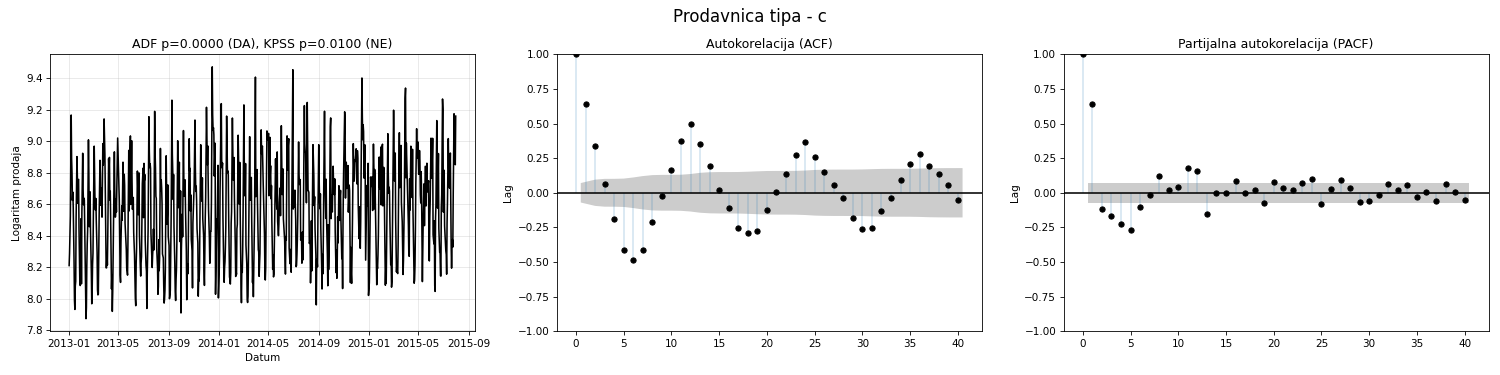
\includegraphics[width=0.9\textwidth]{grafici/store_c.png}
    \vspace{0.3cm}
    
    % Četvrta slika - tip d
    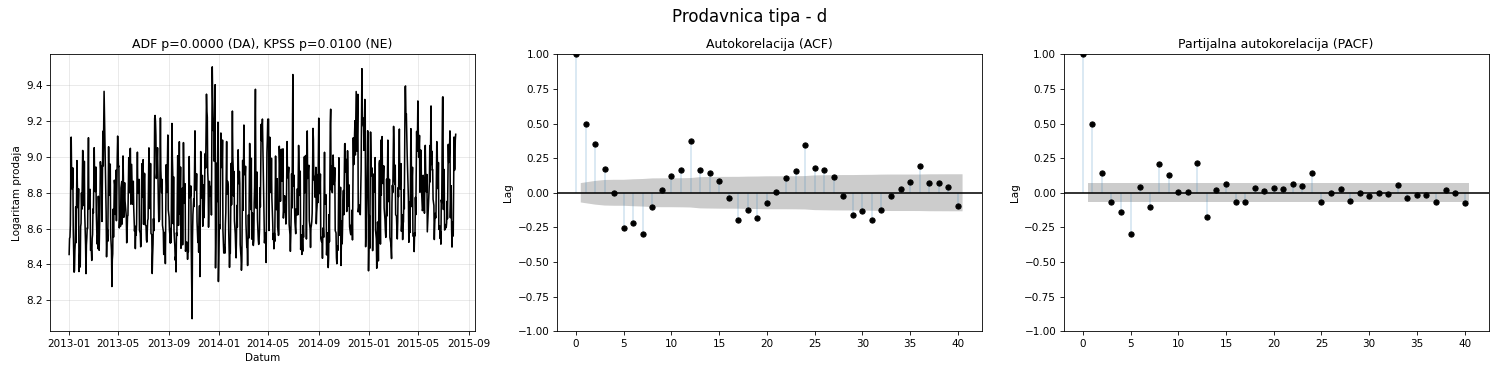
\includegraphics[width=0.9\textwidth]{grafici/store_d.png}
    
    \caption{Vremenski signal, ACF i PACF po tipu prodavnice (\texttt{a}–\texttt{d}).}
    \label{fig:acf_pacf_4x1}
\end{figure}

\subsection{Analiza \textit{outlier}-a} \label{sec:outlier_analysis}

Tokom istraživanja podataka primećeno je da kod 27 prodavnica, u prvim mesecima, postoji značajno odstupajuće ponašanje u odnosu na ostatak serije.  
Ova odstupanja ne mogu se objasniti parametrima dostupnim u skupu podataka.  
Kako bi ovi segmenti podataka mogli negativno uticati na učenje modela, odlučeno je da se uklone iz trenirajućeg skupa.

\begin{figure}[H]
    \centering
    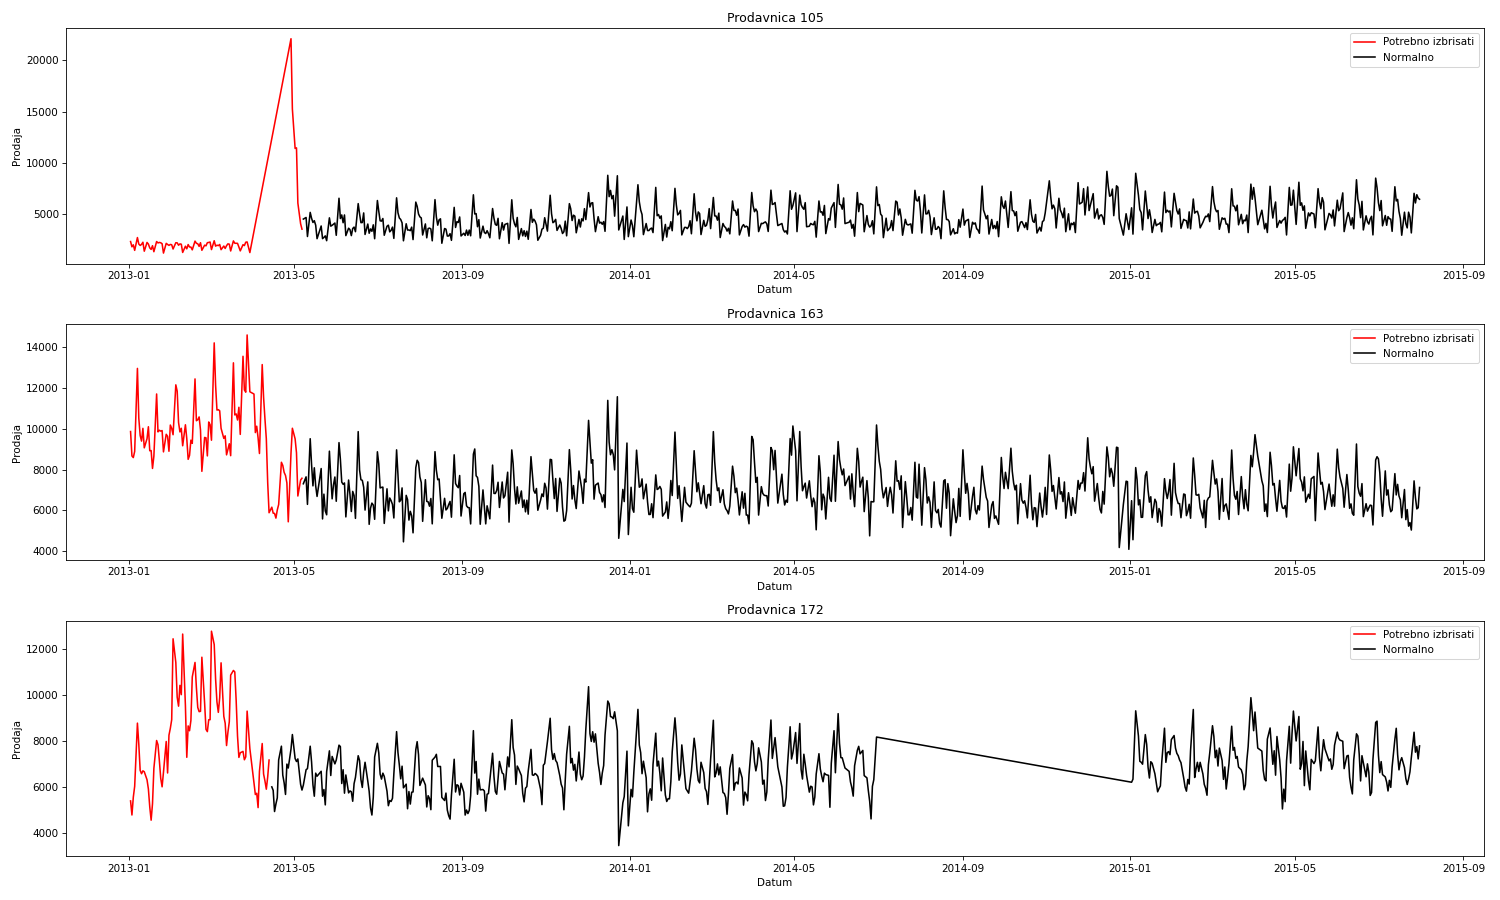
\includegraphics[width=0.9\textwidth]{grafici/outlier_27stores.png}
    \caption{Primeri nekoliko prodavnica sa odstupajućim ponašanjem u početnom periodu.}
    \label{fig:outlier_27stores}
\end{figure}

Pored ovih sistematskih odstupanja, identifikovani su i pojedinačni dani sa izuzetno visokom prodajom koji bi mogli negativno uticati na tačnost predikcije.  
Ovi ekstremni \textit{outlier}-i su detektovani korišćenjem \textit{Median Absolute Deviation} (MAD) pravila sa pragom od 3 standardne devijacije (\(3\sigma\)) primenjenim na distribuciju dnevne prodaje.

\begin{figure}[H]
    \centering
    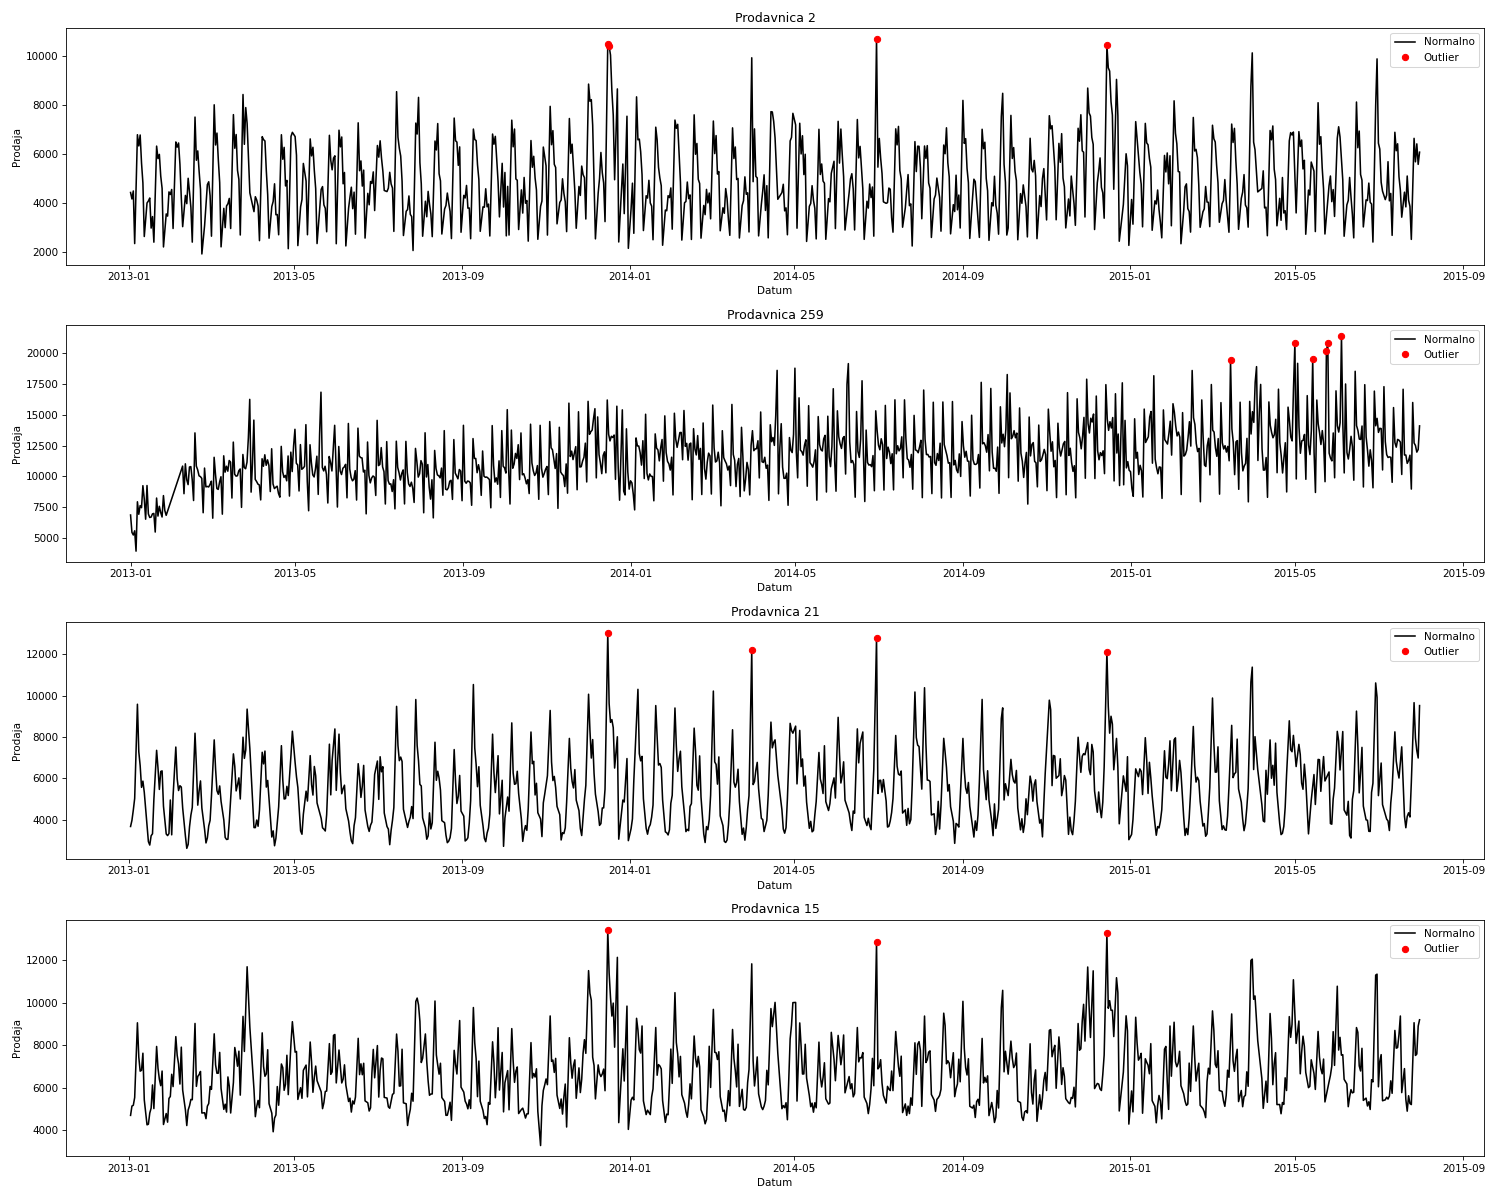
\includegraphics[width=0.9\textwidth]{grafici/extreme_outliers.png}
    \caption{Primeri dana sa ekstremno visokom prodajom.}
    \label{fig:extreme_outliers}
\end{figure}

Pristup obradi outlier-a je sledeći:
\begin{enumerate}
    \item Model je prvobitno treniran bez outlier-a, kako bi se postigla stabilna osnovna procena.
    \item Nedostajući dani sa outlier vrednostima su potom popunjeni predikcijom modela.
    \item Konačni model je treniran na kompletnoj seriji.
\end{enumerate}

\subsection{Korelacija atributa}

Analiza korelacija omogućava uvid u međusobne odnose između promenljivih i njihovu povezanost sa prodajom.  
Posmatrane su samo originalne promenljive iz podataka.  
Na slici~\ref{fig:corr_original} prikazana je korelaciona matrica za ovaj skup atributa.  

Uočava se da je broj kupaca (\texttt{Customers}) ubedljivo najjače povezan sa prodajom (\texttt{Sales}), što je i očekivano.
Ipak, ovaj parametar sam po sebi nije od posebnog značaja za predikciju, jer se broj kupaca ne može unapred znati, već zavisi upravo od faktora koje model nastoji da objasni.
Promotivne aktivnosti (\texttt{Promo}) pokazuju izraženu pozitivnu korelaciju, što potvrđuje povećanje prodaje tokom promotivnih perioda.
S druge strane, prodavnice obuhvaćene dugoročnim programom \texttt{Promo2}, kao što je ranije napomenuto, generalno ostvaruju nižu prosečnu prodaju, pa se kod ovog atributa uočava blaga negativna korelisanost sa prodajom.

Dan u nedelji (\texttt{DayOfWeek}) pokazuje negativnu korelaciju, što je u skladu sa ranijom analizom — prodaja je u proseku najveća početkom nedelje, posebno ponedeljkom.
Takođe, mesec (\texttt{Month}) ostvaruje blagu pozitivnu korelisanost, pre svega zbog povećane prodaje tokom prazničnog perioda u decembru.
Veličina asortimana (\texttt{Assortment}) pokazuje pozitivnu povezanost, jer prodavnice sa bogatijom ponudom proizvoda ostvaruju veći obim prodaje.

\begin{figure}[H]
    \centering
    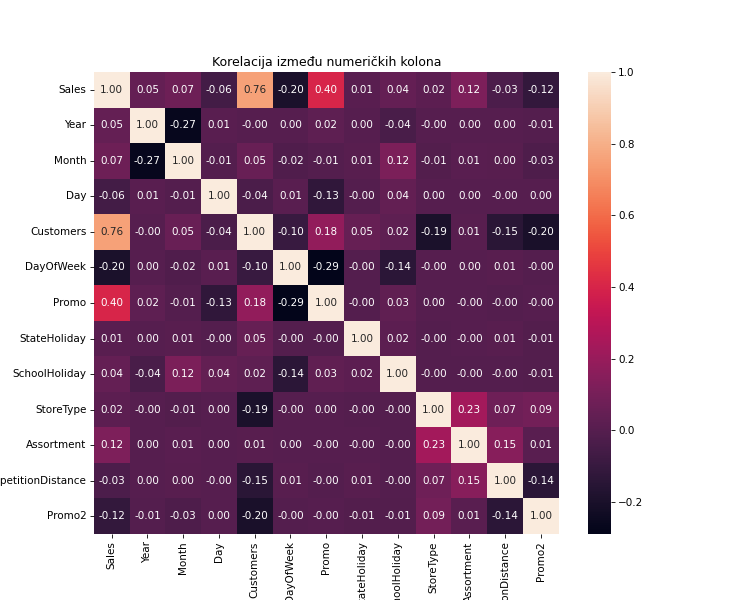
\includegraphics[width=0.9\textwidth]{grafici/correlation_original.png}
    \caption{Korelaciona matrica originalnih atributa.}
    \label{fig:corr_original}
\end{figure}
\newpage
\section{Metodologija i teorijska osnova}

Cilj ovog poglavlja je da predstavi korake i metode korišćene u procesu obrade podataka i izgradnje prediktivnih modela prodaje.  
Proces se sastoji iz tri glavne celine: \textbf{(1)} inženjering osobina (\textit{feature engineering}), \textbf{(2)} korekcija ekstremnih vrednosti (\textit{outlier}-a) i \textbf{(3)} izgradnja i evaluacija modela različite složenosti.

\subsection{Inženjering osobina (Feature Engineering)}

Kako bi se obezbedila što bolja reprezentacija informacija koje utiču na prodaju, nad početnim skupom podataka izvršeno je generisanje dodatnih atributa, transformacija vremenskih karakteristika i kodiranje kategorijskih promenljivih.

Na samom početku, kategorijske promenljive poput tipa prodavnice (\texttt{StoreType}), nivoa asortimana (\texttt{Assortment}) i državnih praznika (\texttt{StateHoliday}) transformisane su primenom jednostavnog ordinalnog kodiranja (\textit{Ordinal Encoder}). Ovim pristupom svaka kategorija dobija numeričku vrednost, čime se omogućava primena modela koji zahtevaju numeričke ulaze.

Zatim su kreirane sledeće dodatne promenljive:

\begin{itemize}
    \item \textbf{Karakteristike konkurencije:} kombinovanjem atributa \texttt{CompetitionOpenSinceYear} i \texttt{CompetitionOpenSinceMonth} izračunat je broj meseci od trenutka kada je konkurencija otvorena – atribut \texttt{CompetitionOpenSince}.

    \item \textbf{Promotivne karakteristike:} iz atributa \texttt{Promo2SinceYear} i \texttt{Promo2SinceWeek} izračunato je koliko nedelja je program \texttt{Promo2} aktivan (\texttt{PromoOpenSince}). Na osnovu atributa \texttt{PromoInterval}, dodata je i binarna promenljiva \texttt{isPromo2}, koja označava da li je prodavnica trenutno uključena u aktivni promotivni ciklus.

    \item \textbf{Praznici:} kreirane su tri binarne promenljive koje označavaju da li se praznik javljao u prethodnoj, tekućoj ili sledećoj nedelji – \texttt{HolidayLastWeek}, \texttt{HolidayThisWeek} i \texttt{HolidayNextWeek}.

    \item \textbf{Zatvaranja prodavnica:} atribut \texttt{ClosureFeat} predstavlja broj dana od poslednjeg zatvaranja prodavnice, čime se modelu omogućava uvid u potencijalni efekat ponovnog otvaranja na prodaju.

    \item \textbf{Statističke karakteristike prodavnica:} za svaku prodavnicu izračunati su:
    \begin{itemize}
        \item prosečna prodaja po danu (\texttt{SalesPerDay}),
        \item prosečan broj kupaca po danu (\texttt{CustomersPerDay}),
        \item prosečna prodaja po kupcu (\texttt{SalesPerCustomers}).
    \end{itemize}
    Ovi indikatori daju modelu uvid u tipično ponašanje svake prodavnice u različitim okolnostima.

    \item \textbf{Pokretne sredine:} uvedene su dve promenljive – \texttt{cond\_mean\_90D} i \texttt{cond\_mean\_365D}, koje predstavljaju prosečnu prodaju tokom poslednjih 90, odnosno 365 dana, pod istim uslovima (prodavnica, aktivnost promocije i tip praznika). Ove vrednosti omogućavaju modelu da koristi lokalne istorijske obrasce kao referencu za očekivanu prodaju.

    \item \textbf{Trend komponente:} za potrebe linearnih modela uveden je trend u vidu broja dana od početka perioda praćenja (\texttt{days\_since\_start}) i njegova logaritamska transformacija (\texttt{log\_days}), koja pomaže u modelovanju dugoročnog rasta prodaje.

    \item \textbf{Sezonske komponente (Furijeove komponente):} radi eksplicitnog hvatanja periodičnih obrazaca u prodaji, dodate su Furijeove komponente različitih perioda i redova:
    \begin{itemize}
        \item nedeljni ciklus (period 7 dana, red 3),
        \item mesečni ciklus (period 12 meseci, red 3),
        \item godišnji ciklus izražen kroz nedelje (period 52 nedelje, red 3),
        \item dugoročni godišnji trend (period 365 dana, red 5).
    \end{itemize}
    Ove komponente su naročito korisne za linearne modele, jer omogućavaju efikasno modelovanje sezonalnosti.

\end{itemize}

Kako bi se proverila informativnost novokreiranih atributa, izračunate su korelacije između novih osobina i ciljane promenljive \texttt{Sales} \ref{fig:corr_engineered}.

\begin{figure}[H]
    \centering
    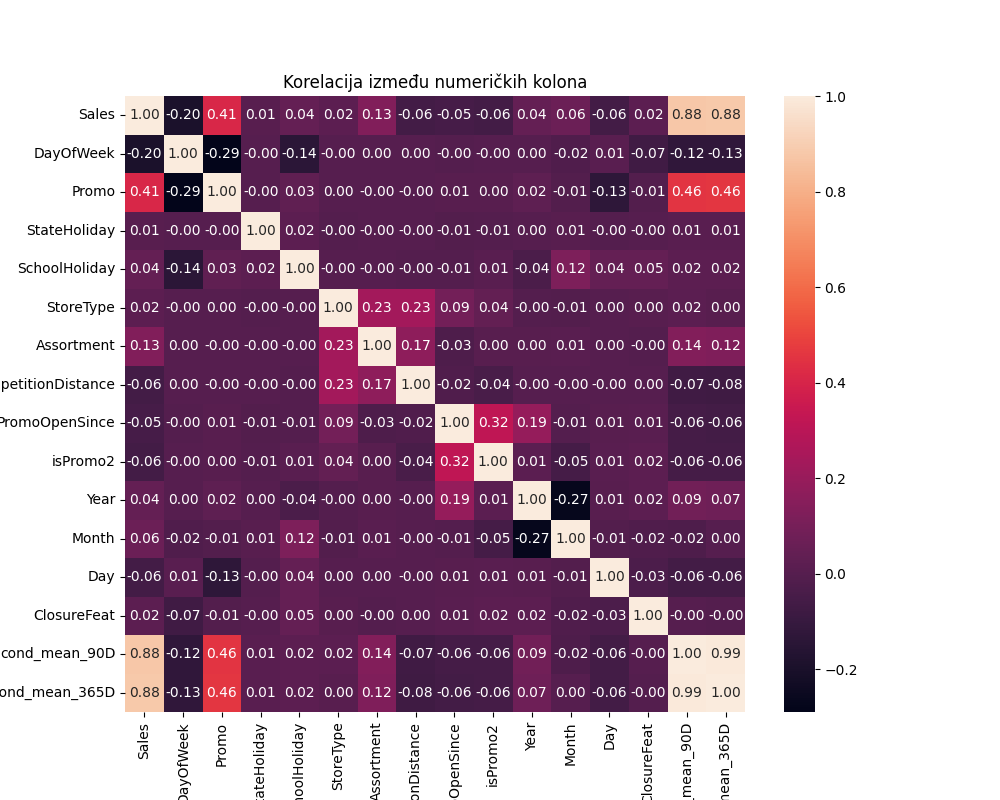
\includegraphics[width=0.9\textwidth]{grafici/correlation_engineered.png}
    \caption{Korelaciona matrica nakon dodavanja generisanih atributa.}
    \label{fig:corr_engineered}
\end{figure}

\newpage
\subsection{Obrada \textit{outlier}-a}

Kao što je detaljno opisano u odeljku \textbf{\ref{sec:outlier_analysis}} \textit{Analiza outlier-a}, u podacima su identifikovane dve grupe anomalija: prodavnice sa neuobičajenim početnim ponašanjem i ekstremne dnevne vrednosti prodaje.  
Kako bi se obezbedilo stabilno učenje modela i sprečilo da ove pojave negativno utiču na tačnost predikcija, sprovedeno je njihova obrada.

\begin{itemize}
    \item \textbf{Prodavnice sa neuobičajenim početnim ponašanjem} – kod 27 objekata uočen je netipičan trend prodaje tokom prvih meseci, bez jasnog uzroka koji bi se mogao objasniti dostupnim atributima. Ti segmenti vremenskih serija su uklonjeni iz skupa podataka pre modeliranja.
    
    \item \textbf{Dnevni ekstremi u prodaji} – Pojedini dani sa neuobičajeno visokim vrednostima prodaje detektovani su korišćenjem \textit{Modified Z-score} metode zasnovane na \textit{median absolute deviation} (MAD) kriterijumu sa pragom od \(3\sigma\).  
Za razliku od standardne devijacije, MAD predstavlja robusniju meru disperzije, jer se zasniva na medijani apsolutnih odstupanja od medijane i samim tim je otpornija na ekstremne vrednosti:

\begin{equation}
    \text{MAD} = \text{median}\left( |x_i - \tilde{x}| \right)
\end{equation}

gde je \(\tilde{x}\) medijana posmatrane promenljive.  
Na osnovu toga, \textit{Modified Z-score} za svaku vrednost \(x_i\) računa se kao:

\begin{equation}
    M_i = \frac{0.6745 \, (x_i - \tilde{x})}{\text{MAD}}
\end{equation}

Vrednosti za koje važi \(|M_i| > 3.5\) smatraju se \textit{outlier}-ima, jer odstupaju više od tri standardne devijacije od centralne distribucije.

\end{itemize}

Nakon što su ekstremne vrednosti detektovane, primenjen je model zasnovan na \textbf{XGBoost}-u (opisan u odeljku \textbf{\ref{subsubsec:xgboost}}) koji je treniran na podacima iz kojih su \textit{outlier}-i prethodno uklonjeni.  
Dobijene predikcije su zatim korišćene za imputaciju tih ekstremnih vrednosti, čime je zadržan kontinuitet vremenske serije bez gubitka informacija.  

Na ovaj način obezbeđeno je da modeli budu trenirani na realističnim, ali stabilizovanim podacima.  
Iako su i nakon korekcije zabeležene pojedine visoke vrednosti prodaje, njihov uticaj na ukupnu strukturu podataka i rezultate modela je značajno smanjen \ref{fig:outlier_correction}.

\begin{figure}[H]
    \centering
    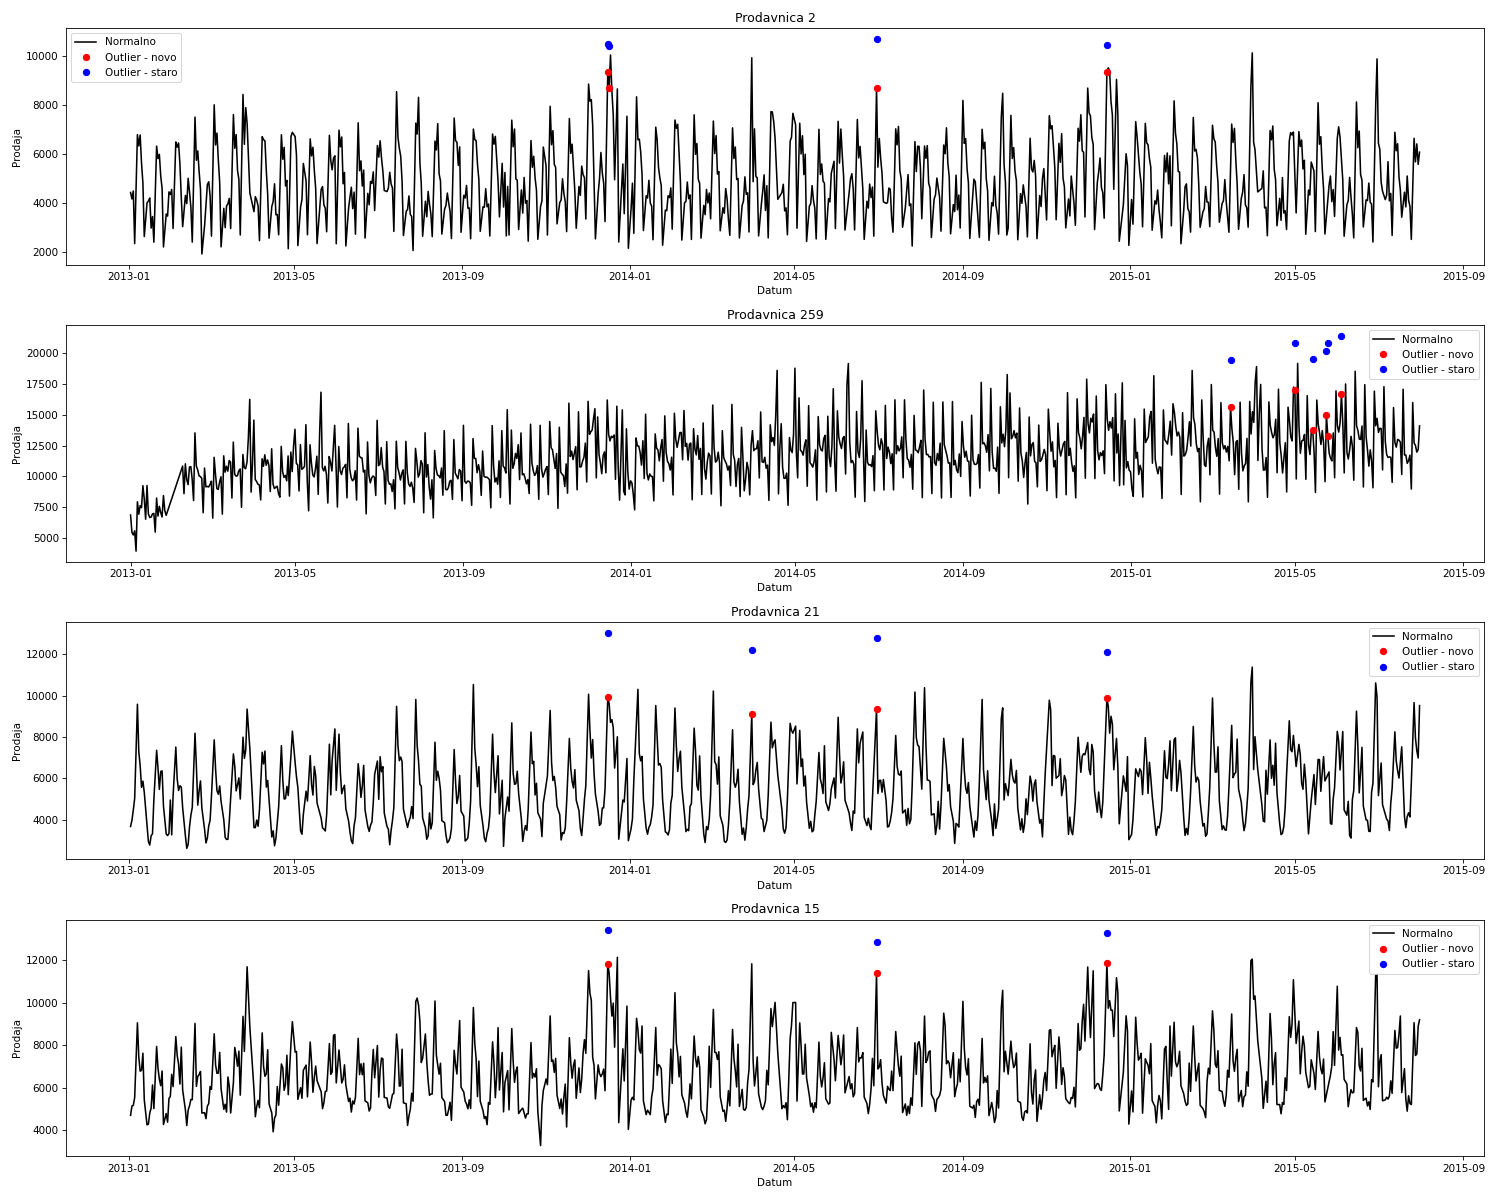
\includegraphics[width=0.9\textwidth]{grafici/outlier_correction.png}
    \caption{Prikaz vremenske serije pre i nakon korekcije ekstremnih vrednosti.}
    \label{fig:outlier_correction}
\end{figure}

\subsection{Modeli predikcije}

U radu su primenjene tri metode predikcije: konstantan model, linearna regresija i XGBoost.

\subsubsection*{Model konstantnog izlaza (bazni model)}

Ovaj model predstavlja najprostiji način predikcije i služi kao referentna tačka.  
Umesto da uči obrasce iz podataka, on za svaku prodavnicu koristi konstantnu vrednost kao predikciju buduće prodaje.  

Za svaku prodavnicu \(s\), konstanta je izračunata kao srednja vrednost svih zabeleženih prodaja u periodu između 1. avgusta i 17. septembra, što odgovara vremenskom intervalu za koji se predviđa buduća prodaja:

\begin{equation}
    \hat{y}_{s} = \frac{1}{N_s} \sum_{i \in \text{train period}} Sales_{i,s}
\end{equation}

gde je \(N_s\) broj dana sa dostupnom prodajom za prodavnicu \(s\).  

Bazni model služi kao osnova za poređenje — složeniji modeli (poput linearne regresije ili XGBoost-a) moraju ostvariti značajno bolje rezultate kako bi se opravdalo njihovo korišćenje.


\subsubsection*{Linearni modeli – Ridge regresija}

Primena \textit{Ridge} regresije omogućava kontrolu nad prekomernim prilagođavanjem modela (\textit{overfitting}) i smanjenje uticaja kolinearnosti između osobina.  
Model je treniran na logaritamski transformisanim vrednostima prodaje (\(\log(1+Sales)\)) kako bi se smanjila asimetrija distribucije i olakšalo učenje linearnog modela.  

Matematički, Ridge regresija rešava problem minimizacije:

\begin{equation}
    \hat{\theta} = \arg\min_\theta \left\{ \sum_{i=1}^{N} \left(y_i - X_i \theta \right)^2 + \alpha \|\theta\|_2^2 \right\},
\end{equation}

gde je \(X\) matrica karakteristika, \(y\) vektor ciljne promenljive (\(\log(1+Sales)\)), \(\theta\) vektor koeficijenata, a \(\alpha\) hiperparametar regularizacije koji kontroliše jačinu penalizacije i smanjuje prevelike koeficijente radi bolje generalizacije.

Rešenje u matricnom obliku glasi:

\begin{equation}
    \hat{\theta} = \left(X^\top X + \alpha I\right)^{-1} X^\top y
\end{equation}

Parametar regularizacije \(\alpha\) odabran je korišćenjem 10\% podataka sa najkasnijim datumima u trening skupu, što omogućava evaluaciju modela na budućim danima i izbor vrednosti koja najbolje generalizuje.

Za eksperimentisanje su korišćena tri pristupa:

\begin{enumerate}
    \item \textbf{Globalno fitovanje} – svi koeficijenti se određuju odjednom za ceo skup podataka. Ovaj pristup je jednostavan, ali daje lošije rezultate zbog ograničenosti modela.
    \item \textbf{Fitovanje po prodavnici} – za svaku prodavnicu posebno se fituju parametri, ali samo za obeležja koji variraju unutar prodavnice, npr. promocije, praznici, vremenska obeležja i Furijeovi redovi. Obeležja koji su konstantni po prodavnici (tip prodavnice, asortiman) se ne koriste u ovom koraku.
    \item \textbf{Hibridni pristup} – prvo se vrši fitovanje po prodavnici da bi se objasnili lokalni obrasci, a preostali reziduali se zatim modeluju globalnim parametrima da bi se iskoristili opšti trendovi.
\end{enumerate}

\subsubsection*{XGBoost model} \label{subsubsec:xgboost}

Za modelovanje nelinearnih odnosa između promenljivih i ciljne varijable korišćen je \textbf{XGBoost} \textit{(Extreme Gradient Boosting)}, ansambl algoritam zasnovan na gradijentnom poboljšavanju stabala odlučivanja.  
Algoritam kombinuje niz \textit{slabih učenika} – stabala odlučivanja – pri čemu svako naredno stablo pokušava da koriguje greške prethodnih (\textit{boosting}), čime se postiže preciznija predikcija.  

Predikcija u iteraciji \(t\) se izražava kao:
\begin{equation}
    \hat{y}^{(t)} = \hat{y}^{(t-1)} + \eta f_t(x),
\end{equation}
gde je \(\eta\) stopa učenja, a \(f_t(x)\) novo stablo koje dodaje korekciju prethodnoj predikciji \(\hat{y}^{(t-1)}\).

Najvažniji hiperparametri uključuju:
\begin{itemize}
    \item \textbf{Broj stabala} – ukupan broj stabala u ansamblu.
    \item \textbf{Maksimalna dubina stabala} – kontroliše složenost stabala.
    \item \textbf{Stopa učenja (\(\eta\))} – doprinos svakog novog stabla.
    \item \textbf{Gamma (\(\gamma\))} – minimalni gubitak potreban za deljenje čvora.
    \item \textbf{Lambda (\(\lambda\)) i Alpha (\(\alpha\))} – L2 i L1 regularizacija, radi kontrole overfitting-a.
\end{itemize}

Optimalni hiperparametri su određeni korišćenjem Bajesovske optimizacije (Optuna), pri čemu je 10\% podataka izdvojeno kao validacioni skup sa najkasnijim datumima, što omogućava procenu performansi na budućim danima.

XGBoost minimizuje sledeću funkciju:

\begin{equation}
    \mathcal{L}(\phi) = \sum_{i=1}^{n} l\left(y_i, \hat{y}_i^{(t-1)} + f_t(x_i)\right) + \Omega(f_t),
\end{equation}

gde je \(l\) funkcija gubitka (u ovom slučaju RMSPE), \(f_t\) novo stablo u iteraciji \(t\), a \(\Omega(f)\) penalizacija složenosti stabla:

\begin{equation}
    \Omega(f) = \gamma T + \frac{1}{2}\lambda \sum_{j=1}^{T} w_j^2 + \alpha \sum_{j=1}^{T} |w_j|,
\end{equation}

pri čemu je \(T\) broj listova stabla, a \(w_j\) težine listova.  


Zbog svoje sposobnosti za nelinearno modelovanje, XGBoost je korišćen kako za globalno modelovanje karakteristika, tako i za modeliranje reziduala nakon uklanjanja sezonalnosti i trenda procenjenih linearno putem Ridge regresije. Time se omogućava da model uči samo neuhvaćene obrasce u podacima.
Kao i kod \textit{Ridge} regresije, za XGBoost je ciljna promenljiva \texttt{Sales} logaritamski transformisana, čime je smanjena asimetrija distribucije i omogućeno stabilnije učenje modela.


\newpage


\section{Rezultati}

Evaluacija modela izvršena je korišćenjem \textbf{RMSPE (Root Mean Square Percentage Error)}:

\begin{equation}
    RMSPE = \sqrt{\frac{1}{N}\sum_{i=1}^{N} \left( \frac{y_i - \hat{y}_i}{y_i} \right)^2 },
\end{equation}

gde su dani sa $y_i = 0$ ignorisani pri izračunavanju.

\begin{table}[H]
\centering
\caption{Poređenje modela po RMSPE}
\begin{tabular}{|l|c|c|c|} % 4 kolone sa vertikalnim linijama
\hline
Model & Tip & Public Score (RMSPE) & Test Score (RMSPE) \\
\hline
Konstantan izlaz & - & 0.27098 & 0.24148 \\
\hline
\multirow{3}{*}{Ridge} 
    & Globalno & 0.19453 & 0.19839 \\ \cline{2-4}
    & Lokalno & 0.11821 & 0.12940 \\ \cline{2-4}
    & Hibridno & 0.11765 & 0.12807 \\
\hline
\multirow{2}{*}{XGBoost} 
    & Globalno & 0.10385 & 0.11321 \\ \cline{2-4}
    & Hibridno & 0.10538 & 0.11440 \\
\hline
\end{tabular}
\end{table}
Iz tabele se vidi da bazni model sa konstantnim izlazom daje najlošije rezultate. Ridge regresija značajno poboljšava preciznost, pri čemu lokalni i hibridni pristup daju bolje rezultate od globalnog fitovanja, dok XGBoost, zahvaljujući sposobnosti modelovanja nelinearnih odnosa i kompleksnih interakcija između atributa, pokazuje najbolje performanse. Neočekivano, hibridni pristup kod Ridge-a daje rezultate vrlo slične lokalnom pristupu, dok hibridni pristup kod XGBoost-a daje rezultate bliske globalnom modelu, što sugeriše da lokalno modelovanje kod Ridge-a već efikasno hvata specifične karakteristike pojedinačnih prodavnica, dok globalni XGBoost uspešno obuhvata opšte obrasce u podacima.

Na slici~\ref{fig:predikcija_example} dat je primer predikcije za jednu prodavnicu korišćenjem konstantnog modela, linearne regresije i XGBoost-a.
\begin{figure}[H]
    \centering
    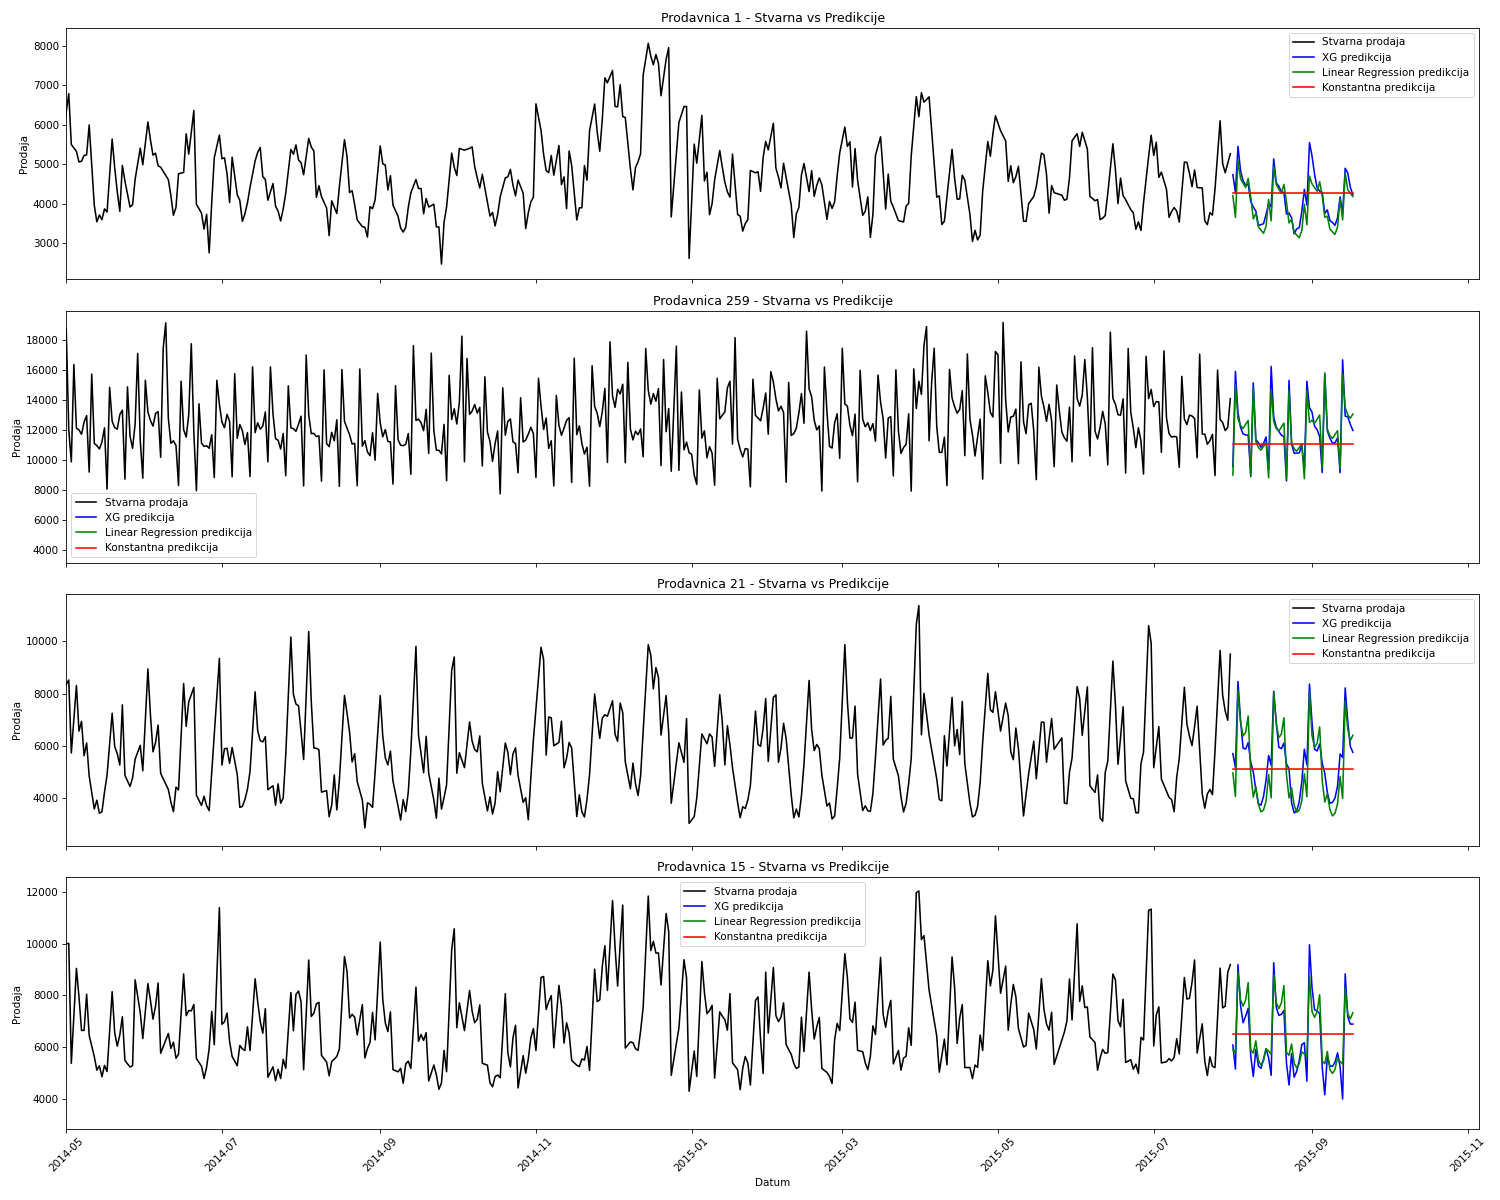
\includegraphics[width=0.8\linewidth]{grafici/prediction_final.png}
    \caption{Predikcije prodaje nekoliko Rossmann prodavnica korišćenjem konstantnog modela, linearne regresije i XGBoost-a.}
    \label{fig:predikcija_example}
\end{figure}


\newpage
\section{Zaključak}

U ovom radu sprovedena je sveobuhvatna analiza vremenskih serija prodaje Rossmann prodavnica, uz cilj da se izgrade modeli sposobni za tačnu predikciju dnevne prodaje.
Primenjeni su i upoređeni različiti pristupi predikciji – od jednostavnog modela sa konstantnim izlazom, preko linearne regresije sa regularizacijom (\textit{Ridge}), do naprednog nelinearnog modela XGBoost.

Rezultati su pokazali da linearni modeli, iako interpretabilni i efikasni, ne mogu u potpunosti uhvatiti kompleksne obrasce sezonalnosti, promocija i interakcija među promenljivama.
XGBoost model se, kao što je i očekivano, pokazao najuspešnijim zahvaljujući mogućnosti modelovanja nelinearnih odnosa.

Dalji koraci mogu obuhvatiti primenu dubokih neuralnih mreža prilagođenih vremenskim serijama, poput LSTM i \textit{Temporal Fusion Transformer} modela, kao i uključivanje dodatnih spoljnih faktora — vremenskih uslova i \textit{Google Trends} podataka — koji bi mogli dodatno poboljšati tačnost predikcije.

Vredno je napomenuti da je pobednički model na zvaničnom Kaggle takmičenju ostvario RMSPE rezultat od 0.10021 na privatnom skupu podataka, koristeći dodatne meteorološke podatke.
Iako je korišćenje takvih informacija bilo dozvoljeno u okviru takmičenja, u realnim uslovima ovakav pristup nije praktičan, jer je teško pouzdano predvideti vremenske prilike šest nedelja unapred, što značajno ograničava primenjivost takvog modela u stvarnim poslovnim scenarijima.

\end{document}
